\documentclass{article}
\usepackage{relsize}
\usepackage{lmodern}
\usepackage{textcomp}
\usepackage{graphicx}
\usepackage{hyperref}
\usepackage[utf8]{inputenc}

\title{The truth about chatbots \\[0.4em]\smaller{}Session n\,°1: Hype and reality}
\author{Louise Crépet}
\date{March 2019}

\begin{document}

\maketitle

\section{Introduction}

The hype cycle is a branded graphical presentation developed and used by Gartner to represent the maturity, adoption, and social application of specific technologies. It’s not really objective, it’s not scientific: the hype cycle is most useful when it’s viewed as descriptive, not prescriptive.\\
There are 5 phases\footnote{\url{https://www.gartner.com/en/research/methodologies/gartner-hype-cycle}}:
\begin{description}
    \item Innovation Trigger: A potential technology breakthrough kicks things off. Early proof-of-concept stories and media interest trigger significant publicity. Often no usable products exist and commercial viability is unproven.
    \item Peak of Inflated Expectations: Early publicity produces a number of success stories — often accompanied by scores of failures. Some companies take action; many do not.
    \item Trough of Disillusionment: Interest wanes as experiments and implementations fail to deliver. Producers of the technology shake out or fail. Investments continue only if the surviving providers improve their products to the satisfaction of early adopters.
    \item Slope of Enlightenment: More instances of how the technology can benefit the enterprise start to crystallize and become more widely understood. Second- and third-generation products appear from technology providers. More enterprises fund pilots; conservative companies remain cautious.
    \item Plateau of Productivity: Mainstream adoption starts to take off. Criteria for assessing provider viability are more clearly defined. The technology's broad market applicability and relevance are clearly paying off.
\end{description}

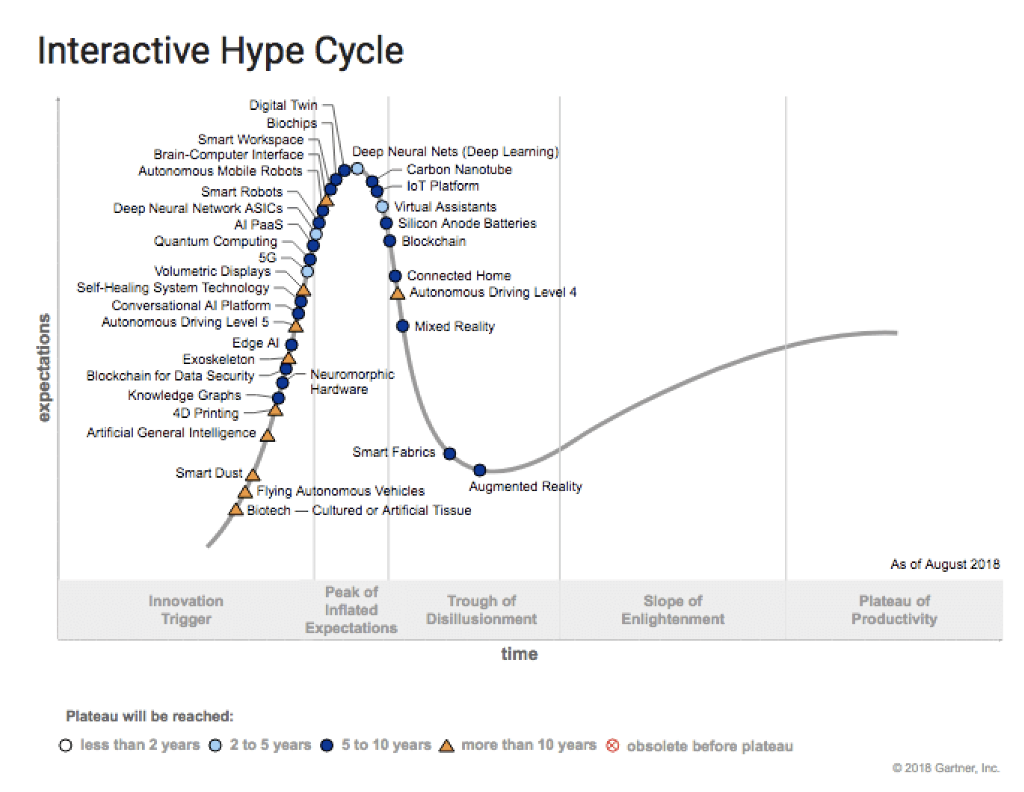
\includegraphics[scale=0.6]{images/hype_cycle.png}
\break
If we look at this representation, we see that the “chatbots” are almost leaving the “Peak of Inflated Expectations”, and are entering the third phase of the cycle: Trough of Disillusionment. It’s the sign we should nuance our very high expectations and take the time to learn from the past experiments and errors.

\section{A bit of context}
What is a "chatbot"? The most known definition is: 
\begin{quote}
A computer program designed to simulate conversation with human users, especially over the Internet. \\
(Oxford Dictionaries)
\end{quote}
It can provide any type of service, from functional to fun, and it can live in any major chat product (Facebook Messenger, Slack, Telegram, WeChat...). 
\break
Chatbot types:
\begin{itemize}  
    \item Customer service: answer to your questions. Ex: Louis (Air France).
    \item Purchasing: allow you to buy things. Ex: Starbucks.
    \item Marketing: try to make you buy things, improve engagement and/or make a brand popular. Ex: NatGeo Genius.
    \item Entertainment: tell jokes, organize quizzes. Ex: Joke Bot.
    \item Informational: push content. Ex: TechCrunch.
\end{itemize}

\section{The climb to the peak}
In the 1960s, Weizenbaum published an innovative study \footnote{\url{http://web.stanford.edu/class/linguist238/p36-weizenabaum.pdf}} on natural language interaction with ELIZA, a computer program developed to simulate conversations by following rules of a script. The most famous script is DOCTOR, allowing ELIZA to mimic the responses of a psychotherapist in a therapy session\footnote{\url{http://psych.fullerton.edu/mbirnbaum/psych101/Eliza.htm}}. It uses pattern matching and substitutions to give the illusion it really talks, while it just asking question about what was said before. It’s interesting to note that you don’t have a real conversation with ELIZA, you are only encouraged to talk; but a lot of people became quite fond of it. The goal was actually to show the superficiality of communication between human and machine.\\
\break
In 1995 came A.L.I.C.E. chatbot\footnote{\url{https://www.pandorabots.com/pandora/talk?botid=b8d616e35e36e881}}, implemented by Dr Wallace. It was able to use natural language processing and therefore to have more sophisticated conversations than ELIZA. Its code is open source, you can find several versions of it on internet\footnote{\url{https://github.com/Crusoe74/alicebot}}. It seems that it was integrated in other chabots to handle the small talk with users.\\
A.L.I.C.E. won the Loebner Prize\footnote{\url{https://www.aisb.org.uk/events/loebner-prize}} in 2000. This annual competition, which exists since 1991, awards prizes to computer programs considered to be the most human-like, even if some of them don't pass the Turing test\footnote{\url{https://en.wikipedia.org/wiki/Turing_test}}. It certainly raised interest of research labs and general public in chatbot technologies in the 1990s.\\
\break
In the beginning of the 2000s, something happened: SmarterChild. It was a chatbot developed by ActiveBuddy and available on AOL Instant Messenger and Windows Live Messenger, former MSN. It was able to handle several tasks, providing news, weather forecasts, sports results... It was also the first instant message chatbot.\\
Chatbots are not just conversation partners anymore: they are now considered as novel marketing tools.\\
\break
The next step was achieved by Apple in 2011 with Siri, the first assistant built natively into an operating system. Google, Amazon and Microsoft followed with Google Assistant, Alexa and Cortana. Assistants’ feature sets were extended into tasks that could be performed across the device’s operating system, instead of inside one application.\\
\break
WeChat is the first messaging app to offer a chatbot platform to its users. Others like Telegram and Slack followed, but none of us had a community big enough to have a big impact.\\
In 2016, Facebook launched its bot API. Like on WeChat, a lot of companies could reach their (potential) customers through Messenger. At the end of 2016, during a keynote presentation at F8, Facebook claimed that 33,000 chatbots were on Messenger.\\
Everybody wanted its chabot. Startups making chatbots popped up everywhere. According to a survey made by Oracle in 2016, 80\% of respondents (composed of 800 “decision makers”) said they already used or planned to use chatbots by 2020\footnote{\url{https://go.oracle.com/LP=43079}}. 

\section{The descent to the trough of disillusionment}

So, why such a disappointment? Actually, chatbots don’t always work well.\\
Let's take a practical example: M. It was the Messenger assistant launched by Facebook in 2015. M was supposed to react to some intents in users’ conversations, insert relevant external links and let chatbots of outside businesses interact with users, like Google Assistant and Alexa are doing. Unfortunately, it wasn't as effective as them. A software engineer working in the Silicon Valley wrote an article about how he found out that humans were behind M, using a kind of "anti-Turing test"\footnote{\url{https://blog.arik.io/facebook-m-the-anti-turing-test-74c5af19987c}}. Facebook admitted later that it could fulfill only about 30\% of requests without human intervention\footnote{\url{https://www.theinformation.com/articles/how-messenger-and-m-are-shifting-gears}}.  In addition, the chatbots built by outside developers were not better and could not understand users requests all the time.\\
M was shut down in 2018, even if the "suggestion" feature, which jumps into conversations on its own, in order to suggest relevant stickers or to offer to schedule a meeting, remains.\\
\break
It’s directly linked to one of the main issue: expectation VS reality. We were so convinced that chatbots could do incredible things, we dreamed so hard that the chatbots would change the world, in short, chabots were so hype that we can hardly handle the fact that chatbots are not as amazing as expected. To be clear: a lot of chatbots are OK, some are really good. But we expect and ask too much of them and the technology didn’t improve as fast as the hype.\\
\break
And we are not helped by some companies that are so excited by this new technology that they
want it everywhere and be the first to be successful. But when you rush, you don’t think, when you don’t think, you do poor stuffs. Chatbots without strong use cases and good design cannot succeed. Making chatbots is not easy. Chatbots are not the magical solution that you can easily launch in two clicks.\\
\break
Sometimes we want to offer to people a solution to a problem they didn’t know they had, or a problem that doesn’t exist. A chatbot is something you have a conversation with, so a chatbot should solve problem that is solved by having a conversation.
Personally, if I want to check the weather, I won’t pick my phone and open Messenger to have a conversation with someone about it, I will pick my phone and look at the Google weather card. A chatbot will never replace an app nor a website.\\
The fact that "everybody" makes a chatbot doesn't mean that is a good idea to build one: a lot of supply is not a lot of demand.\\
\break
Chatbots can’t replace humans neither, for now at least. If I have a car accident, even harmless, the last thing I want to do is send SMS to a bot. A study made in 2017 on 200 requests shows that 40.5\% of these requests were emotional and 59.5\% of them were informational\footnote{\url{https://www.researchgate.net/publication/313204805_A_New_Chatbot_for_Customer_Service_on_Social_Media}}. Chatbots suffer from a lack of empathy and cannot answer properly to an emotional request, so don’t tell your users your chatbot is human: it’s creepy.

\section{What now?}

I won’t lie: maybe building chatbots is a false good idea. Some people think that. But some people thought that “the web” was just a fad 10 years ago.\\
\break
Now that we had a few years to experiment, I think the first question we can ask is: how people use chatbots?\\
\break
These last years, it became more and more simple to post a tweet or a Facebook status to reach a brand than write a detailed email, and the brands receive more and more requests through this channel. A study conducted on 500 respondents on Twitter in 2017 shows that 53\% of users who contact a brand on Twitter expect a response within an hour (72\% if they want to complain). And what do these people when they don’t obtain a quick response? 60\% of them do negative things: escalate their concern through other sources of communication (26\%), consider buying less from the company in the future (24\%), not recommend the company’s products/services (21\%) and shame the company in social media (15\%)\footnote{\url{https://www.lithium.com/company/news-room/press-releases/2013/consumers-will-punish-brands-that-fail-to-respond-on-twitter-quickly}}.\\
The first thing people want is productivity. A chatbot allow them to obtain an answer quickly: they don’t have to have a phone call and wait to  speak to a person or read tons of text. A study about “Why people use chatbots” made in 2017 show that most of the people use chatbots because of the productivity (68\%)\footnote{\url{https://www.researchgate.net/publication/318776998_Why_people_use_chatbots}} because they are so much effective than humans for some tasks.\\
\break
The second thing is convenience: you can talk to a chatbots at anytime of the day and it’s supposed to be always available. In a study conducted by SurveyMonkey in 2017\footnote{\url{https://www.drift.com/wp-content/uploads/2018/01/2018-state-of-chatbots-report.pdf}}, 64\% of the respondents reported the 24-hour service as a potential benefit of the chatbots. It’s  supposed to be easy to “navigate” through information with a chatbot, the search feature is almost free and you can have it on your smartphone. Bots integrated with the apps that are already installed in our devices make easy for us to use services instantly without needing to switch to another platform.\\
\break
And last, people want to be entertained. It can be with an entertaining chatbot but another chatbot can provide a fun and unique user experience.
Entertainment does not exclude productivity; people want to get the job done, but many prefer to do so in an enjoyable manner.\\
\break
These are general data about general users. But each chatbot is a specific case; look at you data: what are the most used scenarios, what the users says to the chatbot, do they give up the conversation and when and why ? Have you already an audience on a specific channel? Does it solve a problem for your customers?\\
\break
You don't build a chatbot because it's possible, but because it's necessary. Ask yourself: what is the purpose and the interest for your business? Faster service and better response times? Accessibility outside opening hours? Create efficiency for service employees by having chatbots prepare the work? Or ensure cost efficiency?
\section{To conclude}
4 takeways:
\begin{itemize}
    \item A chatbot is not suitable for all organizations - and that’s ok.
    \item Chatbots won’t replace humans. They won’t replace apps and websites either.
    \item We still have a lot to do to improve the technology - and it takes time.
    \item Like all the other products and services, the more you know about the needs of the users, the more you can offer a relevant chatbot.
\end{itemize}

\end{document}
